% Modelo de artigo para submissão ao arXiv.
% Compile com: pdflatex main.tex (duas vezes, se necessário).
% Para usar BibTeX, substitua a seção de referências por um arquivo .bib.

\documentclass[11pt,a4paper]{article}

% --- Pacotes básicos ---
\usepackage[utf8]{inputenc}
\usepackage[T1]{fontenc}
\usepackage{lmodern}
\usepackage[english,brazilian]{babel}
\usepackage{microtype}
\usepackage{geometry}
\geometry{margin=1in}

% --- Matemática, figuras e tabelas ---
\usepackage{amsmath,amssymb,mathtools}
\usepackage{graphicx}
\usepackage{booktabs}
\usepackage{url}
\usepackage{siunitx}
\usepackage{xcolor}
\usepackage{graphicx}
\usepackage{subcaption}
\usepackage{float}
% --- Referências e links ---
\usepackage[numbers,sort&compress]{natbib}
\usepackage[hidelinks]{hyperref}
\usepackage[nameinlink,noabbrev]{cleveref}

% --- Configurações ---
\graphicspath{{figures/}}
\hypersetup{
  pdftitle={Avaliação Comparativa de Métodos Neurais de OCR para o Reconhecimento de Palavras Manuscritas em Imagens de Prescrições Médicas},
  pdfauthor={Samuel F. Santos},
  pdfsubject={Artigo científico}
}

% Comandos úteis para manter a notação consistente.
\newcommand{\methodname}{NomeDoMetodo}
\newcommand{\datasetname}{NomeDoConjuntoDeDados}
\newcommand{\TODO}[1]{\textcolor{red}{[TODO: #1]}}

% --- Metadados do artigo ---
%Utilização de diferentes tecnicas de benchmark para reconhecimento de escritas medicas à mão.
\title{Avaliação Comparativa de Métodos Neurais de OCR para o Reconhecimento de Palavras Manuscritas em Imagens de Prescrições Médicas}

\author{
  Samuel F. Santos\thanks{E-mail: lacerdasamuel26@gmail.com}
  \\ Universidade Estadual de Santa Cruz
}

\date{} % Remova esta linha para exibir a data atual.

\begin{document}

\maketitle

\begin{abstract}
Este estudo apresenta uma comparação prática entre modelos baseados em CNN e Transformers para o reconhecimento de palavras manuscritas em imagens de prescrições médicas. Foram avaliados dois conjuntos de dados de origem, o RxHandBD e o Doctor’s Handwritten PrescriptionBD, individualmente e em um cenário de treinamento combinado. O treinamento do zero foi utilizado para uma CNN baseline, formulada como um classificador de palavras em vocabulário fechado, e para um modelo CNN-BiLSTM de reconhecimento sequencial. Já os Transformers pré-treinados TrOCR e PARSeq foram submetidos a fine-tuning para a transcrição de sequências de caracteres. O estudo analisa como as características dos conjuntos de dados, os regimes de treinamento e as diferentes formulações da tarefa afetam o desempenho do reconhecimento, as limitações dos modelos e o custo de treinamento em condições de disponibilidade limitada de dados.\\

This study presents a practical comparison of CNN-based and Transformer-based models for handwritten word recognition in medical prescription images. Two source datasets, RxHandBD and Doctor’s Handwritten PrescriptionBD, were evaluated individually and in a combined training scenario. From-scratch training was used for a CNN baseline formulated as a closed-set word classifier and for a CNN-BiLSTM sequence-recognition model, whereas the pre-trained TrOCR and PARSeq Transformers were fine-tuned for character-sequence transcription. The study examines how dataset characteristics, training regimes, and task formulations affect recognition performance, model limitations, and training cost under limited-data conditions.
\end{abstract}

\noindent\textbf{Keywords:} Neural Network; Convulation; Transformers; Artificial Intelligence.

\section{Introduction}
\label{sec:introduction}

%--Contexto do Problema


%Prescrições Medicas no contexto social

Durante atendimentos médicos, é comum que seja emitida uma prescrição médica contendo informações sobre medicamentos e orientações relacionadas ao tratamento do paciente, com o objetivo de auxiliar na recuperação e na melhoria de seu quadro clínico. Entretanto, o conteúdo dessas prescrições é fortemente influenciado pela caligrafia e pelo contexto em que são elaboradas. Em muitos casos, fatores como a urgência do atendimento e a elevada demanda de pacientes nos ambientes hospitalares impactam diretamente a qualidade da escrita do profissional de saúde.

Como consequência, as prescrições médicas frequentemente apresentam baixo grau de legibilidade, tornando sua interpretação um desafio tanto para farmacêuticos quanto para os próprios pacientes. Essa dificuldade de compreensão levou diversos países e instituições de saúde a adotarem prescrições exclusivamente em formato digital como forma de minimizar erros de interpretação. No entanto, essa abordagem não representa a realidade de todos os contextos, nos quais prescrições manuscritas ainda permanecem amplamente utilizadas. Dessa forma, torna-se relevante investigar e compreender a dificuldade inerente aos caracteres e símbolos de prescrições médicas manuscritas, bem como avaliar a possibilidade de generalizar esse entendimento para outros tipos de escrita manual.


%O que letras medicam descrevem, metalinguagem

Tem-se que, manuscritos tendem a apresentar características relevantes para este estudo, representadas por formas geométricas simplificadas e por estruturas que podem ser compreendidas a partir dos símbolos que compõem a escrita. Dessa forma, as Figuras~\ref{fig:img_a} e~\ref{fig:img_b} evidenciam essas formas básicas, nas quais também são observados ruídos e irregularidades decorrentes das adversidades do ambiente de escrita previamente mencionadas. Assim, essas imagens podem ser utilizadas para a compreensão de padrões geométricos bidimensionais mais complexos, fornecendo uma representação adequada das características estruturais presentes na caligrafia.



\begin{figure}[H]
	\centering
	
	\begin{subfigure}{0.38\textwidth}
		\centering
		
\includegraphics[width=\linewidth]{imagens/prescription.png}
		\caption{}
		\label{fig:img_a}
	\end{subfigure}
	\hfill
	\begin{subfigure}{0.38\textwidth}
		\centering
		
\includegraphics[width=\linewidth]{imagens/rxhandbd.png}
		\caption{}
		\label{fig:img_b}
	\end{subfigure}
	
	\caption{Caracteristicas Geometricas em Prescrições Medicas}
	\label{fig:comparacao}
\end{figure}
%Porque seriam uteis para redes neurais entende-los

No contexto de redes neurais, torna-se relevante avaliar a capacidade de diferentes arquiteturas em compreender e classificar estruturas caligráficas. Esse interesse se justifica tanto pela possibilidade de classificação automática de prescrições médicas quanto pelo potencial de utilização dessas estruturas como base para o aprendizado de representações aplicáveis a problemas envolvendo padrões geométricos de maior complexidade, conforme demonstrado em \cite{ali2024leveraging}. As características geométricas presentes em anotações manuscritas são particularmente relevantes para o treinamento de modelos, pois refletem a naturalidade e a organicidade do contexto em que são produzidas. Além disso, incorporam variações decorrentes da dinâmica da escrita, da individualidade do autor e de influências externas, diferenciando-se de dados sintéticos, que geralmente apresentam padrões mais controlados e menor variabilidade. Dessa forma, o emprego dessas estruturas no treinamento de redes neurais mostra-se útil para o aprendizado de representações mais robustas e com maior capacidade de generalização frente à variabilidade encontrada em cenários reais.


%Porque é problematico (dados, qualidade de imagens, rotulação e coleta)

No entanto, o treinamento de redes neurais com dados provenientes de prescrições médicas enfrenta barreiras relacionadas à escassez de dados, à qualidade das imagens e à rotulação. A escassez de dados decorre da limitada disponibilidade de conjuntos de dados públicos para treinamento, tornando necessária a adoção de técnicas de aumento de dados (\textit{data augmentation}) para ampliar a quantidade de amostras disponíveis. Em relação à qualidade das imagens, esse desafio está associado à idade dos datasets existentes, uma vez que conjuntos de dados mais antigos tendem a apresentar imagens com menor resolução, menor nitidez e maior incidência de artefatos, fatores que devem ser considerados durante o processo de coleta e preparação dos dados. Quanto à rotulação, cada dataset pode apresentar limitações decorrentes de aspectos regionais, não havendo garantia de que um conjunto de dados proveniente dos Estados Unidos, por exemplo, possua as mesmas características caligráficas, terminológicas e estruturais das prescrições médicas brasileiras ou de países europeus. Essas diferenças refletem particularidades linguísticas, culturais e dos próprios sistemas de saúde adotados em cada país. Diante desses desafios, diferentes abordagens foram empregadas ao longo desta pesquisa com o objetivo de minimizar seus impactos e reduzir possíveis prejuízos à qualidade do treinamento e à capacidade de generalização das redes neurais.

%%--Maneiras de solucionar o problema
%%	Para o problema dos dados

Apesar das limitações relacionadas à disponibilidade de dados, este estudo não tem como objetivo realizar uma nova coleta para a construção de um dataset inédito de prescrições médicas. Entretanto, é necessário utilizar uma quantidade adequada de amostras para o treinamento das redes neurais. Para isso, serão aplicadas técnicas de \textit{data augmentation}, com o objetivo de ampliar a diversidade dos dados e aumentar a capacidade de generalização dos modelos.

Serão utilizados dois datasets para o treinamento das redes neurais. Inicialmente, cada dataset será empregado de forma independente, permitindo a avaliação do desempenho dos modelos em cada conjunto de dados. Posteriormente, será realizado um novo treinamento utilizando a combinação dos dois datasets. Essa estratégia busca ampliar a quantidade de amostras disponíveis para treinamento, ao mesmo tempo em que procura reduzir a possibilidade de ocorrência de \textit{overfitting}.

Os datasets selecionados para este estudo foram o RxHandBD \cite{islam2026rxhandbd} e o PrescriptionBD \cite{abdur_rahim_mia_abdullah_al_mamun_abdullah_al_sajid_aurunave_mollik_ruddra_2024}, por apresentarem características adequadas para a tarefa proposta. Após a aplicação das técnicas de aumento de dados e da organização dos conjuntos de treinamento, os dados estarão devidamente preparados para o treinamento das redes neurais.

Para a realização dos experimentos, foram avaliadas quatro arquiteturas de redes neurais, sendo duas baseadas em Redes Neurais Convolucionais (CNNs) e duas baseadas em Transformers. As arquiteturas convolucionais selecionadas foram uma CNN Baseline e uma CNN-BiLSTM, escolhidas por apresentarem menor custo computacional e menor dependência de grandes volumes de dados para treinamento, características compatíveis com o cenário de escassez de dados abordado neste estudo.

As arquiteturas baseadas em Transformers foram o TrOCR e o PARSeq, ambos utilizados a partir de modelos pré-treinados e posteriormente adaptados à tarefa por meio da técnica de \textit{fine-tuning}. Essa abordagem permite aproveitar o conhecimento previamente adquirido durante o pré-treinamento, reduzindo a necessidade de grandes conjuntos de dados específicos para a tarefa.

A avaliação de desempenho foi conduzida considerando as particularidades de cada arquitetura. Dessa forma, as CNNs foram analisadas dentro do contexto de treinamento do zero (\textit{training from scratch}), enquanto os modelos baseados em Transformers foram avaliados no contexto de \textit{fine-tuning}. Assim, as comparações foram realizadas respeitando o cenário de utilização de cada abordagem, evitando comparações diretas que poderiam resultar em interpretações inadequadas devido às diferenças entre seus processos de treinamento.

E para este estudo foi utilizado o hardware da Tabela~\ref{tab:hardware}.

\begin{table}[H]
	\centering
	\caption{Configuração de hardware utilizada nos experimentos.}
	\label{tab:hardware}
	\begin{tabular}{ll}
		\hline
		\textbf{Componente} & \textbf{Especificação} \\ \hline
		Processador (CPU) & Intel Xeon E5-2680 v4 (28 núcleos, 56 threads) \\
		Placa-mãe & MOUGOL X99 \\
		Memória RAM & 8 GB DDR4 \\
		Placa de Vídeo (GPU) & NVIDIA GeForce RTX 3050 Low Profile \\
		Memória de Vídeo (VRAM) & 6 GB \\ \hline
	\end{tabular}
\end{table}

Para a avaliação do desempenho das arquiteturas de redes neurais, foram empregadas diferentes métricas de desempenho, destacando-se a \textit{Word Error Rate} (WER) e a \textit{Character Error Rate} (CER). Além dessas métricas, também foram analisados, ao longo de cada época de treinamento, os valores de perda (\textit{loss}) e de acurácia, permitindo acompanhar a evolução do aprendizado dos modelos.

A análise dessas métricas possibilita avaliar não apenas a capacidade de reconhecimento de palavras e caracteres, mas também identificar a evolução do treinamento, bem como possíveis períodos de estagnação ou convergência. Dessa forma, torna-se possível compreender como as características dos datasets influenciam o desempenho das arquiteturas, contribuindo para a identificação de fatores que favorecem ou limitam a obtenção de melhores resultados.

Diante desse contexto, o objetivo deste estudo é, em um ambiente controlado, avaliar 4 arquiteturas de redes neurais aplicadas ao reconhecimento de prescrições médicas manuscritas. Além disso, busca-se identificar as características dos datasets que influenciam o desempenho de cada arquitetura, analisando quais fatores contribuem para o aumento ou a redução da capacidade de reconhecimento em cada conjunto de dados.


%\section{Related Work}
%\label{sec:related-work}

%presente os trabalhos mais relevantes e explique como este artigo se diferencia
%da literatura. Use citações no formato \citep{exemplo2024} ou \citet{exemplo2024}.

\section{Method}
\label{sec:method}

Para garantir que a comparação entre as arquiteturas fosse conduzida de maneira justa e controlada, este \textit{benchmark} foi estruturado de modo a maximizar a igualdade das condições experimentais entre os dois \textit{datasets}. Com esse objetivo, foi desenvolvido um protocolo de treinamento padronizado, no qual todas as arquiteturas foram submetidas às mesmas configurações de treinamento, incluindo o número de épocas, a taxa de aprendizado (\textit{learning rate}) e o tamanho dos \textit{batches}. Dessa forma, buscou-se minimizar a influência de fatores externos ao processo de treinamento, permitindo que as diferenças observadas nos resultados estivessem predominantemente associadas às características das arquiteturas e dos \textit{datasets} avaliados, tornando a comparação mais consistente e confiável.

Ao término do processo de treinamento, buscou-se consolidar os resultados obtidos por meio de diferentes formas de avaliação. Para isso, foram geradas tabelas contendo as principais métricas de desempenho ao longo do treinamento, além do armazenamento do modelo com melhor desempenho entre todas as épocas. Posteriormente, esse modelo foi submetido à etapa de avaliação, permitindo a obtenção de métricas finais e uma análise consistente de sua capacidade de generalização, fornecendo uma base confiável para a comparação entre as arquiteturas.


\subsection{Proposed Approach}
\label{sec:approach}

A abordagem adotada para a comparação dos modelos consistiu na padronização de todas as etapas experimentais, de modo a garantir condições equivalentes de avaliação. Inicialmente, foi realizado o pré-processamento dos dados, incluindo sua organização e divisão em \textit{splits} de treinamento, validação e teste. Em seguida, os modelos foram desenvolvidos computacionalmente na linguagem Python e treinados utilizando os mesmos hiperparâmetros, assegurando que diferenças de desempenho estivessem relacionadas às arquiteturas avaliadas, e não às configurações de treinamento. Por fim, os modelos foram submetidos ao processo de avaliação, permitindo a comparação sistemática dos resultados obtidos.

\begin{enumerate}
	\item \textbf{Inicialização do modelo:} cada arquitetura foi configurada com
	seus respectivos parâmetros e vocabulário de saída. Para os modelos baseados
	em transformadores, foram utilizados \textit{checkpoints} pré-treinados como
	ponto de partida, enquanto as demais arquiteturas foram instanciadas conforme
	suas definições implementadas.
	
	\item \textbf{Processamento dos dados:} as imagens foram convertidas para
	escala de cinza, redimensionadas para altura de 64 pixels, com largura máxima
	de 512 pixels, preservando-se a razão de aspecto e aplicando-se preenchimento	
	quando necessário. Os rótulos textuais foram normalizados por meio da remoção
	de espaços excedentes e conversão para letras minúsculas. Os dados foram
	organizados em conjuntos fixos de treinamento, validação e teste.
	
	\item \textbf{Otimização:} o treinamento foi realizado em \textit{batches},
	utilizando o otimizador AdamW. A função de perda foi definida de acordo com a
	estratégia de predição de cada arquitetura, incluindo perda por entropia
	cruzada, CTC ou perda baseada em permutações. Ao final de cada época, o
	desempenho no conjunto de validação foi monitorado para selecionar o melhor
	\textit{checkpoint}.
	
	\item \textbf{Avaliação:} o melhor \textit{checkpoint} selecionado na
	validação foi aplicado exclusivamente ao conjunto de teste. O desempenho foi
	quantificado por acurácia de correspondência exata, \textit{Character Error
		Rate} (CER) e \textit{Word Error Rate} (WER), permitindo avaliar tanto a
	correção integral das predições quanto os erros em nível de caracteres e
	palavras.
\end{enumerate}

\section{Experimental Setup}
\label{sec:experiments}

\subsection{Datasets and Preprocessing}
\label{sec:datasets}

O \textit{Doctor's Handwritten Prescription BD Dataset} (\textit{PrescriptionBD}) foi desenvolvido por pesquisadores de Bangladesh com o propósito de disponibilizar um conjunto de dados público voltado ao reconhecimento de prescrições médicas manuscritas~\cite{mia2024deep}. O desenvolvimento do dataset foi motivado pela limitada disponibilidade de bases públicas para o treinamento e a avaliação de modelos de reconhecimento de escrita manuscrita aplicados ao contexto médico. Para sua construção, foram coletadas prescrições médicas reais provenientes de Bangladesh, das quais palavras individuais foram segmentadas e posteriormente anotadas para compor o conjunto de dados. Ao final do processo, o dataset foi disponibilizado publicamente, possibilitando sua utilização em pesquisas relacionadas ao reconhecimento óptico de caracteres (OCR), ao reconhecimento de texto manuscrito (HTR) e a aplicações de inteligência artificial na área da saúde.

A construção do \textit{PrescriptionBD} envolveu procedimentos de segmentação, rotulação e classificação das palavras extraídas das prescrições médicas, resultando em um conjunto de dados organizado e apropriado para o treinamento e a avaliação de modelos de reconhecimento de escrita manuscrita. As amostras apresentam, em geral, boa qualidade visual, com níveis de nitidez que favorecem a extração de características pelas arquiteturas de aprendizado profundo.

Na Figura~\ref{fig:prescriptionbd} são apresentadas algumas amostras do \textit{PrescriptionBD}. Observa-se que o dataset possui imagens com resoluções variáveis, tanto em altura quanto em largura, tornando necessária a realização de uma etapa de padronização para um tamanho único antes do treinamento das redes neurais. Além disso, o \textit{PrescriptionBD} já disponibiliza uma divisão oficial dos dados em conjuntos de treinamento e teste (\textit{train/test split}), característica que contribui para a reprodutibilidade dos experimentos e permite a comparação consistente entre diferentes abordagens.

\begin{figure}[H]
	\centering
	
	\begin{subfigure}{0.15\textwidth}
		\centering
		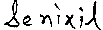
\includegraphics[width=\linewidth]{imagens/211.png}
		\caption{}
		\label{fig:211}
	\end{subfigure}
	\hfill
	\begin{subfigure}{0.15\textwidth}
		\centering
		
\includegraphics[width=\linewidth]{imagens/139.png}
		\caption{}
		\label{fig:139}
	\end{subfigure}
	\hfill
	\begin{subfigure}{0.15\textwidth}
		\centering
		
\includegraphics[width=\linewidth]{imagens/171.png}
		\caption{}
		\label{fig:171}
	\end{subfigure}
	
	\caption{Amostras do PrescriptionBD}
	\label{fig:prescriptionbd}
\end{figure}
	
	

O RxHandBD é um conjunto de dados desenvolvido por Md. Masudul Islam, da Bangladesh University of Business and Technology (BUBT) \cite{islam2026rxhandbd}, e disponibilizado publicamente por meio dos repositórios Zenodo e Mendeley Data. O dataset foi criado com o objetivo de fornecer um benchmark padronizado para pesquisas em reconhecimento de escrita manuscrita (HTR) e reconhecimento óptico de caracteres (OCR) aplicados a prescrições médicas manuscritas.
	
A documentação do \textit{RxHandBD} informa que as amostras foram obtidas a partir de prescrições médicas físicas, das quais palavras individuais foram segmentadas e posteriormente anotadas. No entanto, a documentação disponibilizada não fornece informações detalhadas sobre o processo de aquisição das prescrições, o número de profissionais participantes da coleta, nem os procedimentos empregados para digitalização e segmentação das amostras. O dataset é composto por 5.578 imagens de palavras extraídas de prescrições médicas manuscritas, correspondentes a 1.559 palavras distintas. As imagens são disponibilizadas no formato JPG, enquanto suas respectivas anotações são fornecidas em arquivos CSV.

O \textit{RxHandBD} foi selecionado neste estudo por disponibilizar um conjunto padronizado de palavras provenientes de prescrições médicas manuscritas, contendo transcrições anotadas e uma divisão oficial entre os conjuntos de treinamento e teste. Em comparação ao \textit{PrescriptionBD}, esse dataset apresenta características como maior espessura dos traços das letras e maior expressão da variabilidade regional das caligrafias presentes em prescrições médicas. Essas diferenças tornam o \textit{RxHandBD} um recurso relevante para avaliar a capacidade de generalização dos modelos em cenários com diferentes padrões de escrita manuscrita. Sob uma perspectiva comparativa, é de interesse investigar o desempenho das arquiteturas diante de materiais de escrita com características distintas. Essas particularidades podem ser observadas na Figura~\ref{fig:rxhandbd}, que ilustra exemplos representativos das características caligráficas presentes no dataset.


\begin{figure}[H]
	\centering
	
	\begin{subfigure}{0.15\textwidth}
		\centering
		
\includegraphics[width=\linewidth]{imagens/P0302.jpg}
		\caption{}
		\label{fig:p0302}
	\end{subfigure}
	\hfill
	\begin{subfigure}{0.15\textwidth}
		\centering
		
\includegraphics[width=\linewidth]{imagens/P0163.jpg}
		\caption{}
		\label{fig:p0163}
	\end{subfigure}
		\hfill
	\begin{subfigure}{0.15\textwidth}
		\centering
		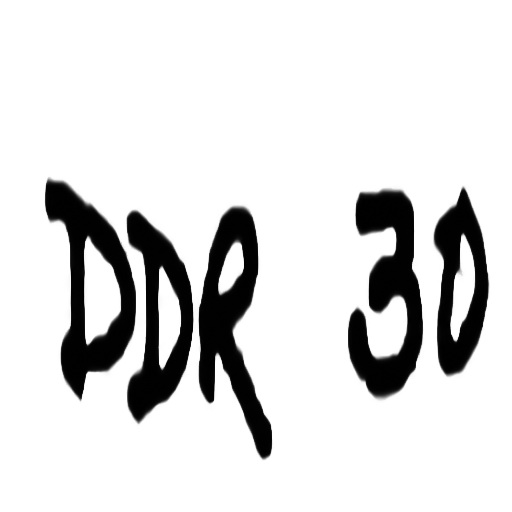
\includegraphics[width=\linewidth]{imagens/P0220.jpg}
		\caption{}
		\label{fig:p0220}
	\end{subfigure}
	
	\caption{Amostras do RxHandBD}
	\label{fig:rxhandbd}
\end{figure}

Conforme discutido anteriormente, o \textit{PrescriptionBD} apresenta imagens com resoluções não padronizadas, cujas dimensões variam tanto em altura quanto em largura. Para garantir a uniformidade do conjunto de dados e possibilitar uma comparação direta com o \textit{RxHandBD}, adotou-se a resolução de ($512 \times 512$) pixels como padrão de entrada para todas as arquiteturas avaliadas. Essa padronização também se faz necessária para a conversão das imagens em tensores de dimensões fixas, requisito fundamental para o treinamento das redes neurais.

Para preservar integralmente o conteúdo das prescrições e evitar distorções geométricas decorrentes de redimensionamentos não proporcionais, optou-se pela técnica de extensão em branco (\textit{padding}). Nesse procedimento, cada imagem foi posicionada sobre um fundo branco até atingir a resolução de ($512 \times 512$) pixels, mantendo suas proporções originais e adicionando apenas pixels de preenchimento nas regiões excedentes. Dessa forma, todas as amostras passaram a apresentar dimensões uniformes, tornando-se adequadas para o processamento pelas arquiteturas de aprendizado profundo e permitindo uma comparação metodológica mais justa entre os datasets. Na Figura~\ref{fig:comp} é possivel ver uma comparação entre imagens antes da padronização e após a padronização, Figura~\ref{fig:stani} é possivel ver a prescrição do medicamento Lenixil em $103\times30$ e na Figura~\ref{fig:512i} após a padronização em $512\times512$.

\begin{figure}[H]
	\centering
	
	\begin{subfigure}{0.4\textwidth}
		\centering
		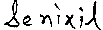
\includegraphics[height=2cm,keepaspectratio]{imagens/211.png}
		\caption{}
		\label{fig:stani}
	\end{subfigure}
	\hspace{1.5cm}
	\begin{subfigure}{0.4\textwidth}
		\centering
		
\includegraphics[height=2cm,keepaspectratio]{imagens/prescriptionbd_test_000212.png}
		\caption{}
		\label{fig:512i}
	\end{subfigure}
	
\caption{Exemplos de imagens do \textit{PrescriptionBD} após a padronização para resolução de $512 \times 512$ pixels.}

	\label{fig:comp}
\end{figure}

Para a realização dos experimentos, foram considerados três cenários distintos: treinamento e avaliação utilizando exclusivamente o \textit{PrescriptionBD}, treinamento e avaliação utilizando exclusivamente o \textit{RxHandBD}, e um cenário adicional composto por um dataset combinado, formado pela união das amostras de ambos os conjuntos de dados. Para esse dataset combinado, foi realizada uma nova divisão entre os conjuntos de treinamento e teste, seguindo os \textit{splits} apresentados na Tabela~\ref{tab:splits}. No caso do \textit{PrescriptionBD}, foi preservada a divisão oficial disponibilizada pelos autores, de modo a garantir a reprodutibilidade dos experimentos e a comparabilidade dos resultados.

\begin{table}[htbp]
	\centering
	\caption{Splits utilizados nos diferentes cenários experimentais.}
	\label{tab:splits}
	\begin{tabular}{lrrrrl}
		\toprule
		\textbf{Cenário} & \textbf{Train} & \textbf{Val} & \textbf{Test} & \textbf{Total} & \textbf{Método} \\
		\midrule
		RxHandBD       & 3905 & 837  & 836  & 5578  & 70/15/15 por amostra, seed 757 \\
		PrescriptionBD & 3120 & 780  & 780  & 4680  & Split oficial preservado \\
		Combinado      & 7025 & 1617 & 1616 & 10258 & União dos splits correspondentes \\
		\bottomrule
	\end{tabular}
\end{table}


Devido à limitada quantidade de amostras disponíveis para treinamento, empregou-se a técnica de \textit{data augmentation} com o objetivo de aumentar a variabilidade dos dados e reduzir o risco de sobreajuste (\textit{overfitting}) dos modelos. As transformações foram aplicadas de forma aleatória durante o treinamento, gerando diferentes variações de uma mesma imagem a cada época.

Foram utilizadas três técnicas de aumento de dados. A primeira consistiu na transformação \textit{RandomAffine}, responsável por aplicar rotações e translações aleatórias às imagens, com probabilidade de $90\%$. A segunda foi a transformação \textit{ColorJitter}, utilizada para modificar aleatoriamente o brilho e o contraste das imagens, com variação de $0{,}25$ para o brilho e $0{,}35$ para o contraste, sendo aplicada com probabilidade de $60\%$. Por fim, empregou-se a transformação \textit{GaussianBlur}, que aplica um desfoque gaussiano utilizando \textit{kernel} de tamanho 3 e valor de $\sigma$ variando entre $0{,}1$ e $0{,}8$, com probabilidade de aplicação de $30\%$. Na Figura~\ref{fig:data-augmentation-examples} é possivel visualizar o resultado da aplicação da metodologia de aumentação em uma amostra do conjunto de dados \textit{RxHandBD}.

\begin{figure}[H]
	\centering
	
	\begin{subfigure}[b]{0.25\textwidth}
		\centering
		\includegraphics[width=\linewidth]{
			imagens/rxhandbd_000001_original.png
		}
		\caption{Imagem original}
		\label{fig:augmentation-original}
	\end{subfigure}
		\vspace{0.8cm}
	\begin{subfigure}[b]{0.25\textwidth}
		\centering
		\includegraphics[width=\linewidth]{
			imagens/rxhandbd_000001_random_affine.png
		}
		\caption{Random Affine}
		\label{fig:augmentation-affine}
	\end{subfigure}
	
	\vspace{0.4cm}
	
	\begin{subfigure}[b]{0.25\textwidth}
		\centering
		\includegraphics[width=\linewidth]{
			imagens/rxhandbd_000001_colorjitter.png
		}
		\caption{ColorJitter}
		\label{fig:augmentation-colorjitter}
	\end{subfigure}
	\vspace{0.8cm}
	\begin{subfigure}[b]{0.25\textwidth}
		\centering
		\includegraphics[width=\linewidth]{
			imagens/rxhandbd_000001_blur.png
		}
		\caption{Desfoque gaussiano}
		\label{fig:augmentation-blur}
	\end{subfigure}
	
	\caption{Exemplo das transformações de data augmentation aplicadas a uma amostra do conjunto de treinamento do RxHandBD.}
	\label{fig:data-augmentation-examples}
\end{figure}

Essas aplicações permitiram um treinamento dos dados mais conciso com menor ocorrência de over-fitting.


\subsection{Computational Models}
\label{sec:models}

Para este projeto foram utilizado 4 arquiteturas, e são elas: Uma CNN baseline, CNN com Bilstm, Trocqr e o Parseq

\subsubsection{CNN Baseline}



As redes neurais convolucionais (\textit{Convolutional Neural Networks} -- CNNs) possuem inspiração em princípios observados no sistema visual biológico, especialmente nos estudos sobre o córtex visual realizados por Hubel e Wiesel \cite{hubel1962receptive}. Embora não representem uma reprodução fiel do funcionamento do cérebro humano, essas arquiteturas foram concebidas a partir da observação de que o sistema visual é capaz de reconhecer padrões complexos por meio da combinação hierárquica de características visuais simples.

Nos experimentos conduzidos por Hubel e Wiesel, observou-se que neurônios presentes no córtex visual respondem seletivamente a estímulos específicos, como bordas, orientações e contrastes. Além disso, verificou-se que o processamento da informação visual ocorre de forma hierárquica, na qual neurônios de níveis superiores integram informações extraídas por neurônios mais simples para representar estruturas cada vez mais complexas \cite{hubel1962receptive}.

Inspiradas nesses princípios, as CNNs introduzem o conceito de campos receptivos locais por meio das camadas de convolução, nas quais filtros aprendem automaticamente padrões presentes nas imagens. À medida que múltiplas camadas convolucionais são empilhadas, torna-se possível construir representações hierárquicas das características visuais, iniciando pela detecção de elementos básicos, como bordas e texturas, e evoluindo para padrões mais complexos, como formas e objetos. Essa organização tornou as CNNs uma das principais arquiteturas para tarefas de visão computacional e reconhecimento de padrões.


Os modelos computacionais das CNNs, tal como são conhecidos atualmente, têm suas bases conceituais no trabalho de Fukushima, apresentado no artigo \textit{Neocognitron: A Self-Organizing Neural Network Model for a Mechanism of Pattern Recognition Unaffected by Shift in Position} \cite{fukushima1980neocognitron}. Nesse estudo foi proposta uma arquitetura hierárquica inspirada no córtex visual, composta por camadas responsáveis pela extração progressiva de características e pela obtenção de invariância a pequenas translações dos padrões de entrada. Embora o Neocognitron não utilizasse treinamento por \textit{backpropagation}, seus princípios arquiteturais serviram de base para o desenvolvimento das CNNs modernas.

Posteriormente, LeCun et al. \cite{lecun1998gradient} consolidaram esse paradigma ao apresentar uma arquitetura convolucional treinada por \textit{backpropagation} para reconhecimento óptico de caracteres (OCR), demonstrando que a aprendizagem automática de filtros convolucionais possibilitava elevados níveis de desempenho em tarefas de reconhecimento de padrões. Esse trabalho estabeleceu as bases práticas para a ampla adoção das CNNs em problemas de visão computacional.

Esta CNN foi utilizada neste projeto como um modelo de referência (\textit{baseline}), representando o ponto de partida para a comparação entre as arquiteturas avaliadas. Seu emprego permite estabelecer um desempenho inicial para modelos convolucionais tradicionais em tarefas de reconhecimento de prescrições médicas manuscritas, servindo como base para a análise dos ganhos proporcionados por arquiteturas mais sofisticadas.

Entretanto, o problema abordado neste trabalho difere de uma tarefa convencional de classificação de imagens. O objetivo consiste em reconhecer palavras completas presentes nas prescrições, caracterizando um problema de reconhecimento de sequências. Uma CNN convencional realiza apenas uma única classificação para cada imagem de entrada, o que a impede de predizer diretamente todos os caracteres que compõem uma palavra em uma única inferência.

Para contornar essa limitação, a CNN \textit{baseline} foi modelada como um classificador de palavras. Nessa abordagem, cada palavra presente no conjunto de treinamento é tratada como uma classe distinta. Consequentemente, a saída da rede corresponde a uma distribuição de probabilidades sobre todas as classes conhecidas, sendo selecionada como predição a palavra com maior probabilidade. Dessa forma, o modelo não realiza o reconhecimento sequencial dos caracteres, mas estima diretamente a qual palavra previamente aprendida a imagem de entrada pertence.

Como evolução da CNN \textit{baseline}, foi desenvolvida uma arquitetura que incorpora uma camada \textit{Bidirectional Long Short-Term Memory} (BiLSTM). Essa modificação permite que o modelo deixe de realizar apenas a classificação de palavras previamente conhecidas e passe a reconhecer a sequência de caracteres presente na imagem, tornando-o mais adequado para tarefas de reconhecimento de texto manuscrito.

\newpage
\subsubsection{CNN BiLSTM}

Posteriormente, visando aumentar a precisão do reconhecimento, foi incorporado um módulo de \textit{Bidirectional Long Short-Term Memory} (BiLSTM) à CNN baseline. Essa arquitetura consiste em uma rede neural recorrente capaz de modelar dependências sequenciais de longo alcance, processando a sequência simultaneamente nos sentidos direto e inverso \cite{shi2016crnn}. Dessa forma, o modelo passa a considerar não apenas o elemento atual, mas também o contexto fornecido pelos caracteres anteriores e posteriores.

A inclusão do BiLSTM justifica-se pelo fato de palavras manuscritas apresentarem uma estrutura sequencial inerente. Em um idioma, determinados caracteres possuem maior probabilidade de ocorrer em conjunto, como a frequente alternância entre consoantes e vogais, além de padrões ortográficos característicos de cada palavra. Ao explorar essas dependências contextuais, o BiLSTM complementa as características visuais extraídas pela CNN, permitindo que a classificação considere tanto a aparência dos caracteres quanto a relação sequencial existente entre eles. Assim, a arquitetura CNN-BiLSTM foi avaliada quanto à sua capacidade de melhorar o reconhecimento de prescrições médicas manuscritas em comparação à CNN baseline.

Com a incorporação do BiLSTM, a arquitetura passou a produzir saídas temporais e foi treinada com CTC sobre um vocabulário de caracteres. Na decodificação gulosa, repetições consecutivas e o símbolo de preenchimento (\textit{blank}) são removidos para reconstruir a palavra predita. Assim, diferentemente da CNN \textit{baseline}, a CNN-BiLSTM não ficou restrita a um conjunto fechado de classes de palavras e pode formar sequências não observadas durante o treinamento, desde que seus caracteres pertençam ao vocabulário aprendido.

Para ampliar a comparação com arquiteturas sequenciais inicializadas a partir de pré-treinamento em larga escala, foram posteriormente avaliados modelos baseados em \textit{Transformers}. Esses modelos também realizam o reconhecimento em nível de sequência de caracteres e podem reconhecer palavras que não estavam presentes no conjunto de treinamento.


\subsubsection{TrOCR}

O TrOCR (Transformer-based Optical Character Recognition) é um modelo de reconhecimento óptico de caracteres proposto por Li et al \cite{li2023trocr}. que utiliza uma arquitetura encoder-decoder baseada inteiramente em Transformers. O modelo emprega um Transformer visual para extrair representações da imagem de entrada e um Transformer textual para gerar a sequência correspondente de caracteres ou tokens, eliminando a necessidade de arquiteturas tradicionais baseadas em CNN, RNN e CTC. Além disso, o TrOCR pode ser pré-treinado em grandes conjuntos de dados sintéticos e posteriormente ajustado com dados rotulados, apresentando aplicação em textos impressos, manuscritos e presentes em cenas naturais.

\subsubsection{PARSeq}

O PARSeq (Permuted Autoregressive Sequence) é um modelo baseado em Transformers desenvolvido para reconhecimento de texto em imagens, especialmente no contexto de Scene Text Recognition \cite{bautista2022parseq}. Diferentemente de modelos autoregressivos convencionais, que geram os caracteres seguindo apenas a ordem da esquerda para a direita, o PARSeq utiliza Permutation Language Modeling, permitindo que o modelo aprenda diferentes ordens de predição e explore contexto bidirecional durante o reconhecimento. Essa abordagem possibilita combinar inferência autoregressiva, não autoregressiva e refinamento iterativo em uma única arquitetura, oferecendo bom equilíbrio entre precisão, número de parâmetros e custo computacional.

\subsection{Baselines and Metrics}
\label{sec:baselines}

Para a realização das comparações entre as arquiteturas, foi inicialmente definida uma matriz de experimentos, responsável por estabelecer os conjuntos de treinamento e de teste utilizados em cada modelo. Essa padronização permitiu conduzir avaliações sistemáticas por meio de métricas consistentes, possibilitando analisar o desempenho de cada arquitetura e compreender os fatores que influenciaram os resultados obtidos. Ao final, os resultados de todos os experimentos foram comparados entre si.

Com o objetivo de garantir uma comparação justa entre as arquiteturas, foram definidas matrizes de comparação específicas para cada conjunto de experimentos. Essas matrizes consideram as diferenças conceituais entre os modelos, bem como suas particularidades de treinamento, evitando comparações inadequadas entre abordagens distintas. Dessa forma, foi possível avaliar a capacidade de generalização e o desempenho de cada arquitetura em diferentes cenários e quantidades de dados disponíveis para treinamento.

É possivel visualizar todos os experiemntos na Tabela~\ref{tab:matriz-experimentos}.
\begin{table}[H]
	\centering
	\caption{Matriz de experimentos por arquitetura e conjunto de dados.}
	\label{tab:matriz-experimentos}
	\begin{tabular}{cllrrr}
		\toprule
		\textbf{Exp.} &
		\textbf{Arquitetura} &
		\textbf{Dataset} &
		\textbf{Treino} &
		\textbf{Validação} &
		\textbf{Teste} \\
		\midrule
		
		E1 & CNN baseline & PrescriptionBD & 3120 & 780  & 780  \\
		E1 & CNN baseline & RxHandBD       & 3905 & 837  & 836  \\
		E1 & CNN baseline & Combinado      & 7025 & 1617 & 1616 \\
		\midrule
		
		E2 & CNN-BiLSTM   & PrescriptionBD & 3120 & 780  & 780  \\
		E2 & CNN-BiLSTM   & RxHandBD       & 3905 & 837  & 836  \\
		E2 & CNN-BiLSTM   & Combinado      & 7025 & 1617 & 1616 \\
		\midrule
		
		E3 & TrOCR        & PrescriptionBD & 3120 & 780  & 780  \\
		E3 & TrOCR        & RxHandBD       & 3905 & 837  & 836  \\
		E3 & TrOCR        & Combinado      & 7025 & 1617 & 1616 \\
		\midrule
		
		E4 & PARSeq       & PrescriptionBD & 3120 & 780  & 780  \\
		E4 & PARSeq       & RxHandBD       & 3905 & 837  & 836  \\
		E4 & PARSeq       & Combinado      & 7025 & 1617 & 1616 \\
		\bottomrule
	\end{tabular}
\end{table}

Ao longo de todo o processo de treinamento foram coletadas métricas referentes ao desempenho do modelo em cada época, com o objetivo de compreender a evolução do aprendizado durante o treinamento. Para isso, foram registrados os valores da função de perda (*loss*) nos conjuntos de treinamento e validação, bem como a acurácia obtida em ambos os conjuntos.

Para a avaliação dos modelos, foram utilizadas métricas capazes de analisar diferentes aspectos do desempenho no reconhecimento de texto. A acurácia foi empregada para medir a capacidade do modelo de reconhecer corretamente toda a sequência de caracteres presente em uma imagem. Além disso, foi utilizada a métrica \textit{Character Error Rate} (CER), que quantifica a taxa de erros em nível de caractere, indicando o número de inserções, deleções e substituições necessárias para transformar a predição no texto de referência. Complementarmente, foi utilizada a métrica \textit{Word Error Rate} (WER), que avalia os erros em nível de palavra, medindo a quantidade de palavras reconhecidas incorretamente em relação ao texto esperado.

\subsection{Implementation Details}
\label{sec:implementation}

Os experimentos foram implementados em Python utilizando o pacote desenvolvido
neste projeto, denominado \texttt{med-ocr-research}. O ambiente de execução
utiliza Python 3.10 ou superior e tem como principal framework de aprendizado
profundo o PyTorch. Todos os treinamentos foram executados com aceleração CUDA
em uma GPU NVIDIA GeForce RTX 3050 com 6 GB de memória. A configuração completa
do ambiente computacional pode ser visualizada na
Tabela~\ref{tab:hardware}.

As principais dependências utilizadas durante o desenvolvimento são
apresentadas na Tabela~\ref{tab:software}. Os valores apresentados representam
as versões mínimas utilizadas no ambiente experimental. Para o TrOCR, os
arquivos do modelo pré-treinado registram a utilização da biblioteca
Transformers na versão 5.12.1.

\begin{table}[htbp]
	\centering
	\caption{Dependências de software utilizadas no ambiente experimental.}
	\label{tab:software}
	\begin{tabular}{llll}
		\toprule
		\textbf{Biblioteca} & \textbf{Versão} &
		\textbf{Biblioteca} & \textbf{Versão} \\
		\midrule
		Python            & $\geq 3.10$   & PyTorch          & $\geq 2.2$  \\
		Torchvision       & $\geq 0.17$   & Transformers     & 5.12.1       \\
		NumPy             & $\geq 1.24$   & Pandas           & $\geq 2.0$  \\
		Pillow            & $\geq 10.0$   & Timm             & $\geq 1.0$  \\
		PyTorch Lightning & $\geq 2.2$    & Accelerate       & $\geq 0.30$ \\
		Albumentations    & $\geq 1.4$    & SentencePiece    & $\geq 0.2.1$ \\
		NLTK              & $\geq 3.8$    & Tqdm             & $\geq 4.66$ \\
		PyYAML            & $\geq 6.0$    & Protobuf         & $\geq 4.25$ \\
		\bottomrule
	\end{tabular}
\end{table}

Durante todos os experimentos foi utilizada a semente aleatória 42 para garantir
a reprodutibilidade dos resultados. Essa semente foi aplicada aos geradores das
bibliotecas \texttt{random}, NumPy e PyTorch, incluindo a inicialização da CUDA
por meio de \texttt{torch.cuda.manual\_seed\_all}. Para a organização dos
datasets foi preservado o split oficial do PrescriptionBD. Já para o RxHandBD,
foi realizada uma divisão de 70\% para treinamento, 15\% para validação e 15\%
para teste, utilizando a semente derivada 757. O dataset combinado foi obtido
por meio da união dos respectivos subconjuntos dos dois datasets.

A CNN Baseline e a CNN-BiLSTM foram implementadas computacionalmente neste
projeto. Para o TrOCR foi utilizado o checkpoint pré-treinado
\texttt{microsoft/trocr-small-handwritten}. Já para o PARSeq foi utilizada a
implementação disponibilizada no repositório \texttt{baudm/parseq}, fixada no
commit \texttt{1902db043c029a7e03a3818c616c06600af574be}. Todo o código-fonte
desenvolvido, bem como as configurações experimentais e os scripts de avaliação,
estão disponíveis no repositório do projeto:

\begin{center}
	\url{https://github.com/SamuelFerrc/Medical-Handwriting-Ocr}
\end{center}


\section{Results and Discussion}
\label{sec:results}

Esta seção reúne os resultados das doze avaliações realizadas: quatro famílias
de modelos, cada uma avaliada nos datasets PrescriptionBD, RxHandBD e no cenário
combinado. A ordem foi organizada para permitir a discussão em três níveis:
(i) comparação agregada entre modelos, (ii) efeito do dataset e (iii) análise
diagnóstica de cada avaliação. As métricas foram recalculadas diretamente a
partir dos arquivos de predições avaliadas. As tabelas detalhadas permanecem
disponíveis na pasta de artefatos para consulta, mas não são inseridas no artigo
principal para manter a seção de resultados concisa.

\subsection{Overall comparison}
\label{sec:results-overall}

A comparação agregada por modelo e cenário é apresentada nas Figuras~\ref{fig:comparison-accuracy},
\ref{fig:comparison-cer} e~\ref{fig:comparison-wer}, que mostram, respectivamente,
a acurácia de correspondência exata, o CER e o WER para as doze avaliações.

Além dos gráficos, a Tabela~\ref{tab:evaluation-summary-all} apresenta as
métricas agregadas de cada modelo e cenário em formato compacto.

\input{tabelas/evaluation_graficos_tabelas/evaluation_summary_all.tex}

\begin{figure}[H]
  \centering
  \includegraphics[width=0.94\linewidth]{imagens/evaluation_graficos_tabelas/comparison_all_evaluations_accuracy.png}
  \caption{Exact-match accuracy across all twelve evaluations.}
  \label{fig:comparison-accuracy}
\end{figure}

\begin{figure}[H]
  \centering
  \includegraphics[width=0.94\linewidth]{imagens/evaluation_graficos_tabelas/comparison_all_evaluations_cer.png}
  \caption{Character Error Rate (CER) across all twelve evaluations.}
  \label{fig:comparison-cer}
\end{figure}

\begin{figure}[H]
  \centering
  \includegraphics[width=0.94\linewidth]{imagens/evaluation_graficos_tabelas/comparison_all_evaluations_wer.png}
  \caption{Word Error Rate (WER) across all twelve evaluations.}
  \label{fig:comparison-wer}
\end{figure}

Os resultados vistos na Figura~\ref{fig:comparison-accuracy} demonstraram que os modelos apresentaram unanimemente melhor desempenho no conjunto de dados PrescriptionBD. Esse comportamento, entretanto, não foi observado no RxHandBD, no qual a maioria dos modelos obteve desempenho inferior, com exceção da CNN Baseline, que apresentou resultados relativamente mais consistentes.

Essa diferença pode ser atribuída principalmente às características visuais de cada conjunto de dados. Conforme ilustrado na Figura~\ref{fig:rxhandbd}, as imagens do RxHandBD apresentam traços mais espessos, borrados e com menor definição, dificultando a extração de características discriminativas tanto pelas CNNs quanto pelos modelos baseados em Transformers. Em contrapartida, a Figura~\ref{fig:prescriptionbd} mostra que o PrescriptionBD possui caracteres com traços mais finos, contínuos e bem definidos, favorecendo a identificação de padrões e a aprendizagem de representações mais robustas pelas redes neurais. Consequentemente, as diferenças na qualidade visual dos conjuntos de dados exerceram influência direta no desempenho dos modelos durante o treinamento e a inferência.

Por sua vez, os experimentos realizados sobre o conjunto de dados combinado apresentaram desempenho intermediário em relação aos dois conjuntos originais. Esse comportamento era esperado, uma vez que o conjunto combinado reúne simultaneamente as características favoráveis do PrescriptionBD e os desafios presentes no RxHandBD. Dessa forma, os modelos foram expostos tanto a exemplos de maior qualidade quanto a amostras com maior complexidade visual, resultando em um desempenho médio entre os dois cenários avaliados.

Uma característica notável foi que a CNN-BiLSTM apresentou um CER menor no conjunto de dados RxHandBD do que no PrescriptionBD, conforme observado na Figura~\ref{fig:comparison-cer}. Esse resultado indica que, apesar de o RxHandBD representar um conjunto de dados mais desafiador para a maioria dos modelos avaliados, a arquitetura CNN-BiLSTM foi capaz de reconhecer os caracteres individuais com maior precisão nesse cenário específico.

Em todos os modelos e conjuntos de dados avaliados, o WER apresentou comportamento consistente com a acurácia geral, conforme ilustrado na Figura~\ref{fig:comparison-wer}. De maneira geral, modelos que obtiveram maiores valores de acurácia também apresentaram menores valores de WER, evidenciando uma relação inversa entre essas métricas e reforçando a consistência dos resultados experimentais.

\subsection{Dataset-specific comparison}
\label{sec:results-dataset}

Para separar o efeito do cenário combinado do efeito da arquitetura, a
Figura~\ref{fig:comparison-combined-dataset} apresenta visualmente, por dataset,
a comparação de acurácia, CER e WER.

\begin{figure}[H]
  \centering
  \includegraphics[width=0.94\linewidth]{imagens/evaluation_graficos_tabelas/comparison_combined_by_dataset.png}
  \caption{Comparison of the combined scenario by dataset.}
  \label{fig:comparison-combined-dataset}
\end{figure}

Para cada modelo de rede neural, foi calculada a diferença entre os resultados representados pelas barras azul e laranja, em relação a acurácia geral. A CNN Baseline foi o único modelo em que a barra laranja apresentou desempenho superior à barra azul, com uma diferença de 7,3 pontos percentuais. Nos demais modelos, a barra azul obteve desempenho superior, apresentando diferenças de 18,2 pontos percentuais para a CNN-BiLSTM, 15,9 pontos percentuais para o TrOCR e 18,4 pontos percentuais para o PARSeq.

\subsection{Per-evaluation diagnostic views}
\label{sec:results-diagnostics}

As figuras desta subseção complementam as métricas agregadas. Cada painel de
predições avaliadas reúne distribuição de erros, relação entre desempenho e
comprimento da referência e acurácia por faixa de confiança. O painel por
rótulo mostra a distribuição de desempenho entre palavras, destacando os
rótulos mais frequentes e os rótulos com menor acurácia. Esses painéis são
descritivos e devem ser usados para investigar padrões de erro, não como
substitutos das métricas agregadas.

\subsubsection{CNN baseline}

\begin{figure}[H]
  \centering
  \begin{subfigure}{0.49\linewidth}
    \centering
    \includegraphics[width=\linewidth]{imagens/evaluation_graficos_tabelas/e1.01cnn_evaluation_evaluated_predictions.png}
    \caption{Evaluated predictions.}
  \end{subfigure}\hfill
  \begin{subfigure}{0.49\linewidth}
    \centering
    \includegraphics[width=\linewidth]{imagens/evaluation_graficos_tabelas/e1.01cnn_evaluation_per_label_metrics.png}
    \caption{Per-label metrics.}
  \end{subfigure}
  \caption{CNN baseline evaluated on PrescriptionBD.}
  \label{fig:diagnostic-e1-prescriptionbd}
\end{figure}

\begin{figure}[H]
  \centering
  \begin{subfigure}{0.49\linewidth}
    \centering
    \includegraphics[width=\linewidth]{imagens/evaluation_graficos_tabelas/e1.02cnn_evaluation_evaluated_predictions.png}
    \caption{Evaluated predictions.}
  \end{subfigure}\hfill
  \begin{subfigure}{0.49\linewidth}
    \centering
    \includegraphics[width=\linewidth]{imagens/evaluation_graficos_tabelas/e1.02cnn_evaluation_per_label_metrics.png}
    \caption{Per-label metrics.}
  \end{subfigure}
  \caption{CNN baseline evaluated on RxHandBD.}
  \label{fig:diagnostic-e1-rxhandbd}
\end{figure}

\begin{figure}[H]
  \centering
  \begin{subfigure}{0.49\linewidth}
    \centering
    \includegraphics[width=\linewidth]{imagens/evaluation_graficos_tabelas/e1.03cnn_evaluation_evaluated_predictions.png}
    \caption{Evaluated predictions.}
  \end{subfigure}\hfill
  \begin{subfigure}{0.49\linewidth}
    \centering
    \includegraphics[width=\linewidth]{imagens/evaluation_graficos_tabelas/e1.03cnn_evaluation_per_label_metrics.png}
    \caption{Per-label metrics.}
  \end{subfigure}
  \caption{CNN baseline evaluated in the combined scenario.}
  \label{fig:diagnostic-e1-combined}
\end{figure}

\subsubsection{CNN-BiLSTM}

\begin{figure}[H]
  \centering
  \begin{subfigure}{0.49\linewidth}
    \centering
    \includegraphics[width=\linewidth]{imagens/evaluation_graficos_tabelas/e2.01_e2cnn_bilstm_evaluation_evaluated_predictions.png}
    \caption{Evaluated predictions.}
  \end{subfigure}\hfill
  \begin{subfigure}{0.49\linewidth}
    \centering
    \includegraphics[width=\linewidth]{imagens/evaluation_graficos_tabelas/e2.01_e2cnn_bilstm_evaluation_per_label_metrics.png}
    \caption{Per-label metrics.}
  \end{subfigure}
  \caption{CNN-BiLSTM evaluated on PrescriptionBD.}
  \label{fig:diagnostic-e2-prescriptionbd}
\end{figure}

\begin{figure}[H]
  \centering
  \begin{subfigure}{0.49\linewidth}
    \centering
    \includegraphics[width=\linewidth]{imagens/evaluation_graficos_tabelas/e2.02_e2cnn_bilstm_evaluation_evaluated_predictions.png}
    \caption{Evaluated predictions.}
  \end{subfigure}\hfill
  \begin{subfigure}{0.49\linewidth}
    \centering
    \includegraphics[width=\linewidth]{imagens/evaluation_graficos_tabelas/e2.02_e2cnn_bilstm_evaluation_per_label_metrics.png}
    \caption{Per-label metrics.}
  \end{subfigure}
  \caption{CNN-BiLSTM evaluated on RxHandBD.}
  \label{fig:diagnostic-e2-rxhandbd}
\end{figure}

\begin{figure}[H]
  \centering
  \begin{subfigure}{0.49\linewidth}
    \centering
    \includegraphics[width=\linewidth]{imagens/evaluation_graficos_tabelas/e2.03_e2cnn_bilstm_evaluation_evaluated_predictions.png}
    \caption{Evaluated predictions.}
  \end{subfigure}\hfill
  \begin{subfigure}{0.49\linewidth}
    \centering
    \includegraphics[width=\linewidth]{imagens/evaluation_graficos_tabelas/e2.03_e2cnn_bilstm_evaluation_per_label_metrics.png}
    \caption{Per-label metrics.}
  \end{subfigure}
  \caption{CNN-BiLSTM evaluated in the combined scenario.}
  \label{fig:diagnostic-e2-combined}
\end{figure}

\subsubsection{TrOCR}

\begin{figure}[H]
  \centering
  \begin{subfigure}{0.49\linewidth}
    \centering
    \includegraphics[width=\linewidth]{imagens/evaluation_graficos_tabelas/e3.01_trocr_evaluation_evaluated_predictions.png}
    \caption{Evaluated predictions.}
  \end{subfigure}\hfill
  \begin{subfigure}{0.49\linewidth}
    \centering
    \includegraphics[width=\linewidth]{imagens/evaluation_graficos_tabelas/e3.01_trocr_evaluation_per_label_metrics.png}
    \caption{Per-label metrics.}
  \end{subfigure}
  \caption{TrOCR evaluated on PrescriptionBD.}
  \label{fig:diagnostic-e3-prescriptionbd}
\end{figure}

\begin{figure}[H]
  \centering
  \begin{subfigure}{0.49\linewidth}
    \centering
    \includegraphics[width=\linewidth]{imagens/evaluation_graficos_tabelas/e3.02_trocr_evaluation_evaluated_predictions.png}
    \caption{Evaluated predictions.}
  \end{subfigure}\hfill
  \begin{subfigure}{0.49\linewidth}
    \centering
    \includegraphics[width=\linewidth]{imagens/evaluation_graficos_tabelas/e3.02_trocr_evaluation_per_label_metrics.png}
    \caption{Per-label metrics.}
  \end{subfigure}
  \caption{TrOCR evaluated on RxHandBD.}
  \label{fig:diagnostic-e3-rxhandbd}
\end{figure}

\begin{figure}[H]
  \centering
  \begin{subfigure}{0.49\linewidth}
    \centering
    \includegraphics[width=\linewidth]{imagens/evaluation_graficos_tabelas/e3.03_trocr_evaluation_evaluated_predictions.png}
    \caption{Evaluated predictions.}
  \end{subfigure}\hfill
  \begin{subfigure}{0.49\linewidth}
    \centering
    \includegraphics[width=\linewidth]{imagens/evaluation_graficos_tabelas/e3.03_trocr_evaluation_per_label_metrics.png}
    \caption{Per-label metrics.}
  \end{subfigure}
  \caption{TrOCR evaluated in the combined scenario.}
  \label{fig:diagnostic-e3-combined}
\end{figure}

\subsubsection{PARSeq}

\begin{figure}[H]
  \centering
  \begin{subfigure}{0.49\linewidth}
    \centering
    \includegraphics[width=\linewidth]{imagens/evaluation_graficos_tabelas/e4.01_parseq_evaluation_evaluated_predictions.png}
    \caption{Evaluated predictions.}
  \end{subfigure}\hfill
  \begin{subfigure}{0.49\linewidth}
    \centering
    \includegraphics[width=\linewidth]{imagens/evaluation_graficos_tabelas/e4.01_parseq_evaluation_per_label_metrics.png}
    \caption{Per-label metrics.}
  \end{subfigure}
  \caption{PARSeq evaluated on PrescriptionBD.}
  \label{fig:diagnostic-e4-prescriptionbd}
\end{figure}

\begin{figure}[H]
  \centering
  \begin{subfigure}{0.49\linewidth}
    \centering
    \includegraphics[width=\linewidth]{imagens/evaluation_graficos_tabelas/e4.02_parseq_evaluation_evaluated_predictions.png}
    \caption{Evaluated predictions.}
  \end{subfigure}\hfill
  \begin{subfigure}{0.49\linewidth}
    \centering
    \includegraphics[width=\linewidth]{imagens/evaluation_graficos_tabelas/e4.02_parseq_evaluation_per_label_metrics.png}
    \caption{Per-label metrics.}
  \end{subfigure}
  \caption{PARSeq evaluated on RxHandBD.}
  \label{fig:diagnostic-e4-rxhandbd}
\end{figure}

\begin{figure}[H]
  \centering
  \begin{subfigure}{0.49\linewidth}
    \centering
    \includegraphics[width=\linewidth]{imagens/evaluation_graficos_tabelas/e4.03_parseq_evaluation_evaluated_predictions.png}
    \caption{Evaluated predictions.}
  \end{subfigure}\hfill
  \begin{subfigure}{0.49\linewidth}
    \centering
    \includegraphics[width=\linewidth]{imagens/evaluation_graficos_tabelas/e4.03_parseq_evaluation_per_label_metrics.png}
    \caption{Per-label metrics.}
  \end{subfigure}
  \caption{PARSeq evaluated in the combined scenario.}
  \label{fig:diagnostic-e4-combined}
\end{figure}

\section{Limitations}
\label{sec:limitations}

Este trabalho apresentou limitações relacionadas à quantidade de dados utilizada e ao tamanho dos \textit{batches} de treinamento, restritos pela capacidade de memória disponível. Essas limitações podem ter introduzido algum viés nos resultados obtidos. Entretanto, todos os modelos foram treinados e avaliados sob as mesmas condições experimentais, utilizando o mesmo ambiente computacional e configurações de treinamento, de forma a garantir a maior equidade possível na comparação entre os métodos.


\section{Conclusion}
\label{sec:conclusion}

Os resultados obtidos evidenciam o potencial dos modelos de reconhecimento sequencial para a transcrição de palavras manuscritas em prescrições médicas. Em particular, TrOCR e PARSeq alcançaram os melhores desempenhos entre os métodos avaliados, com vantagens consistentes em relação à CNN baseline nos três cenários experimentais. O PARSeq destacou-se no PrescriptionBD, atingindo $90{,}13\%$ de acurácia, CER de $0{,}0680$ e WER de $0{,}1000$, enquanto o TrOCR apresentou o melhor desempenho global no cenário combinado em acurácia ($80{,}88\%$) e WER ($0{,}2018$). Esses resultados mostram que o uso de modelos pré-treinados, adaptados por \textit{fine-tuning}, constitui uma estratégia eficaz para OCR de escrita médica manuscrita mesmo em um cenário de disponibilidade limitada de dados.

\section*{Code and Data Availability}

O código, os dados e os materiais suplementares estão disponíveis em:
\url{https://github.com/SamuelFerrc/Medical-Handwriting-Ocr}. 

\bibliographystyle{unsrtnat}
\bibliography{references}
\end{document}
